%%
%% Class homework & solution template for latex
%% Alex Ihler
%%
\documentclass[twoside,11pt]{article}
\usepackage{amsmath,amsfonts,amssymb,amsthm}
\usepackage{graphicx,color}
\usepackage{verbatim,url}
\usepackage{listings}
\usepackage{subcaption} 
\usepackage{upquote}
\usepackage[T1]{fontenc}
%\usepackage{lmodern}
\usepackage[scaled]{beramono}
%\usepackage{textcomp}

% Directories for other source files and images
\newcommand{\bibtexdir}{../bib}
\newcommand{\figdir}{fig}

\newcommand{\E}{\mathrm{E}}
\newcommand{\Var}{\mathrm{Var}}
\newcommand{\N}{\mathcal{N}}
\newcommand{\matlab}{{\sc Matlab}\ }

\setlength{\textheight}{9in} \setlength{\textwidth}{6.5in}
\setlength{\oddsidemargin}{-.25in}  % Centers text.
\setlength{\evensidemargin}{-.25in} %
\setlength{\topmargin}{0in} %
\setlength{\headheight}{0in} %
\setlength{\headsep}{0in} %

\renewcommand{\labelenumi}{(\alph{enumi})}
\renewcommand{\labelenumii}{(\arabic{enumii})}

\theoremstyle{definition}
\newtheorem{MatEx}{M{\scriptsize{ATLAB}} Usage Example}

\definecolor{comments}{rgb}{0,.5,0}
\definecolor{backgnd}{rgb}{.95,.95,.95}
\definecolor{string}{rgb}{.2,.2,.2}
\lstset{language=Matlab}
\lstset{basicstyle=\small\ttfamily,
        mathescape=true,
        emptylines=1, showlines=true,
        backgroundcolor=\color{backgnd},
        commentstyle=\color{comments}\ttfamily, %\rmfamily,
        stringstyle=\color{string}\ttfamily,
        keywordstyle=\ttfamily, %\normalfont,
        showstringspaces=false}
\newcommand{\matp}{\mathbf{\gg}}




\begin{document}

\centerline{\Large Homework 4}
\centerline{Zachary DeStefano, 15247592}
\centerline{CS 274B: Spring 2016}

This is the code I used. After some trial and error, I settled on a step size of $0.01$ yet my results were still not as expected. 

\section*{Code}


\begin{lstlisting}

num_iter = 10
num_points_per_iter = len(files)
stepSize = 0.01
lambdaVal = 0.01
totalPts = num_iter*num_points_per_iter

hammingLossValues = np.zeros(totalPts)
hammingLossAfterIter = np.zeros(num_iter)
hingeLossValues = np.zeros(totalPts)
hingeLossAfterIter = np.zeros(num_iter)

index = 0
perSymHingeLoss = 0
perSymHammingLoss = 0

for iter in range(num_iter):
    randomInds = np.random.permutation(len(files))
    randomIndsUse = randomInds[0:num_points_per_iter]
    for s in  randomIndsUse:
        # Load data ys,xs
        fh = open(datapath + files[s], 'r')
        rawlines = fh.readlines()
        lines = [line.strip('\n').split(',') for line in rawlines]
        fh.close()
        ys = [int(l[1]) - 1 for l in lines]
        xs = [[int(l[2]) - 1, int(l[3]), int(l[4]), int(l[5]) - 1, int(l[6]) - 1] for l in lines]

        ns = len(ys)

        #Define random variables for the inference process:
        Y = [gm.Var(i,10) for i in range(ns)]

				#Construct the factors for prediction
        factors = []
        for ii in range(ns):
            curTable = np.matrix(np.zeros((10,1)))
            for ff in range(len(feature_sizes)):
                curTh = np.matrix(ThetaF[ff])
                curX = xs[ii][ff]
                curMat = np.matrix(curTh[:,curX])
                curTable = np.add(curTable,curMat)

            if ii<(ns-1):
                curMat = np.matrix(ThetaP[:,ys[ii+1]])
                curMat = np.reshape(curMat,(10,1))
                curTable = np.add(curTable,curMat)
								
            factors.append(gm.Factor([Y[ii]],curTable).exp())

        model_pred = gm.GraphModel(factors)

        # Copy factors and add extra Hamming factors for loss-augmented model
        factors_aug = [ f for f in factors ]
        factors_aug.extend( [gm.Factor([Y[i]], Loss[:,ys[i]]).exp() for i in range(ns)] )
        model_aug = gm.GraphModel(factors_aug)

        order = range(ns) # eliminate in sequence (Markov chain on y)
        wt = 1e-4 # for max elimination in JTree implementation

        # Now, the most likely configuration of the prediction model (for prediction) is:
        yhat_pred = gm.wmb.JTree(model_pred,order,wt).argmax()
				yhatVals = yhat_pred.values()
				
        # and the maximizing argument of the loss (for computing the gradient) is
        yhat_aug = gm.wmb.JTree(model_aug,order,wt).argmax()
        yhatAugVals = yhat_aug.values()

        # use yhat_pred & ys to keep a running estimate of your prediction accuracy & print it
        #... # how often etc is up to you
        yhatVals = yhat_pred.values()
        hammingLoss = 0
        accuracy = 0
        for ii in range(ns):
            if(abs(yhatVals[ii]-ys[ii])>=1):
                hammingLoss += 1
            else:
                accuracy +=1
        print np.divide(np.double(accuracy),np.double(ns)) #print the accuracy

        #calculate hinge loss factors
        hingeLoss = 0
        hingeLoss += hammingLoss
        for ii in range(ns):
            for ff in range(len(feature_sizes)):
                curTh = np.matrix(ThetaF[ff])
                curX = xs[ii][ff]
                diffFactor = curTh[yhatAugVals[ii],curX]-curTh[ys[ii],curX]
                hingeLoss += diffFactor

            if ii < (ns - 1):
                otherDiff = ThetaP[yhatAugVals[ii], ys[ii + 1]]-ThetaP[ys[ii], ys[ii + 1]]
                hingeLoss += otherDiff
        for ii in range(10):
            for jj in range(10):
                hingeLoss += lambdaVal*(ThetaP[ii,jj]**2)
        for ff in range(numFeats):
            for ii in range(10):
                for jj in range(feature_sizes[ff]):
                    hingeLoss += lambdaVal*(ThetaF[ff][ii,jj]**2)
										
        # use yhat_aug & ys to update your parameters theta in the negative gradient direction
        for ii in range(ns-1):
            ThetaP[yhatAugVals[ii], yhatAugVals[ii + 1]] -= stepSize
            ThetaP[ys[ii],ys[ii+1]] += stepSize
        ThetaP = ThetaP - stepSize*lambdaVal * ThetaP

        for ii in range(ns):
            for ff in range(numFeats):
                ThetaF[ff][yhatAugVals[ii],xs[ii][ff]] -= stepSize
                ThetaF[ff][ys[ii], xs[ii][ff]] += stepSize
        for ff in range(numFeats):
            ThetaF[ff] = ThetaF[ff] - stepSize*lambdaVal * ThetaF[ff]

        perSymHingeLoss = np.divide(np.double(hingeLoss),np.double(ns))
        perSymHammingLoss = np.divide(np.double(hammingLoss), np.double(ns))
        hingeLossValues[index] = perSymHingeLoss
        hammingLossValues[index] = perSymHammingLoss
        index += 1

\end{lstlisting}

\newpage

\section*{Results}

For the first attempt, I did 10 passes through a random 100 points in each pass. The Hamming Loss seemed to decrease stochastically yet the Hinge Loss exhibited significant variance. I then tried 2 passes through all 6000 points and the Hinge Loss still exhibited the variance. The Hamming Loss seemed to stochatically decrease in the first 2000 points.

\begin{figure}[h]
\centering
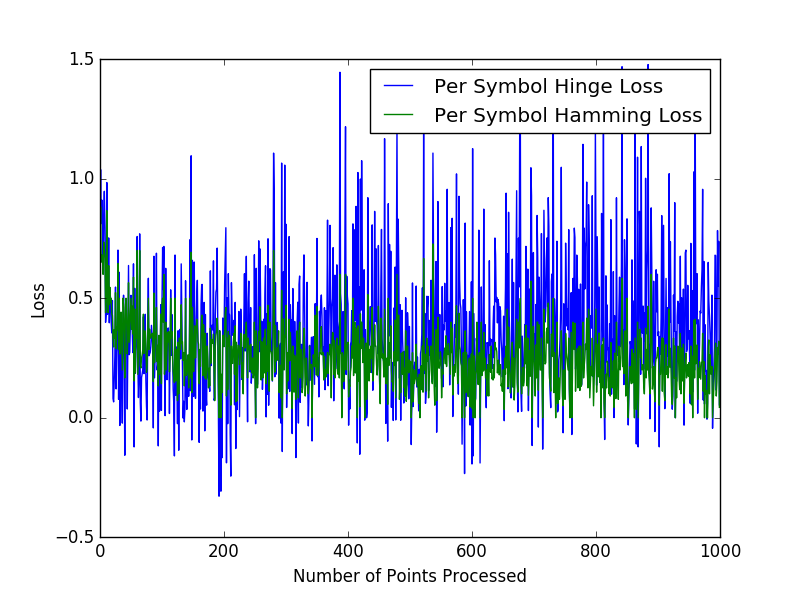
\includegraphics[width=5in]{hingeHammingLoss1.png}
\caption{Hinge and Hamming Loss for 10 passes with 100 points each pass}
\end{figure}

\begin{figure}[h]
\centering
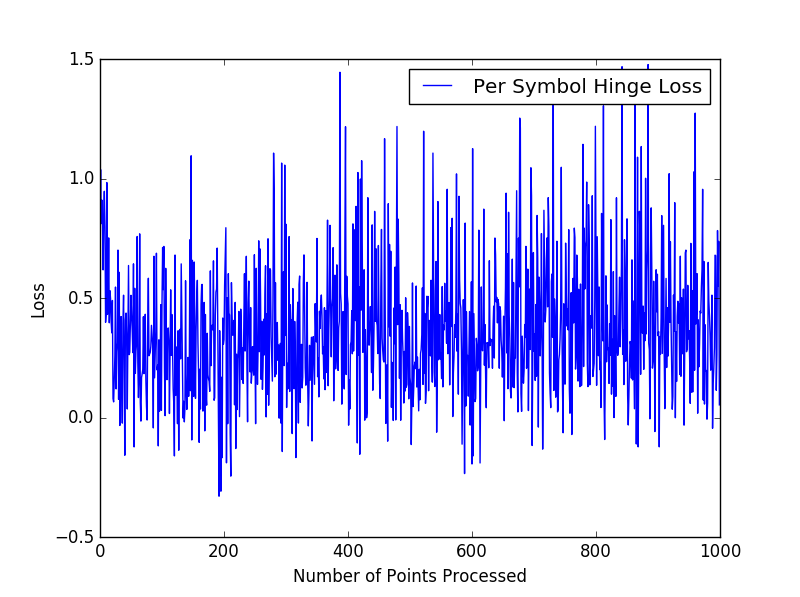
\includegraphics[width=5in]{hingeLoss1.png}
\caption{Hinge Loss for 10 passes with 100 points each pass}
\end{figure}

\begin{figure}[h]
\centering
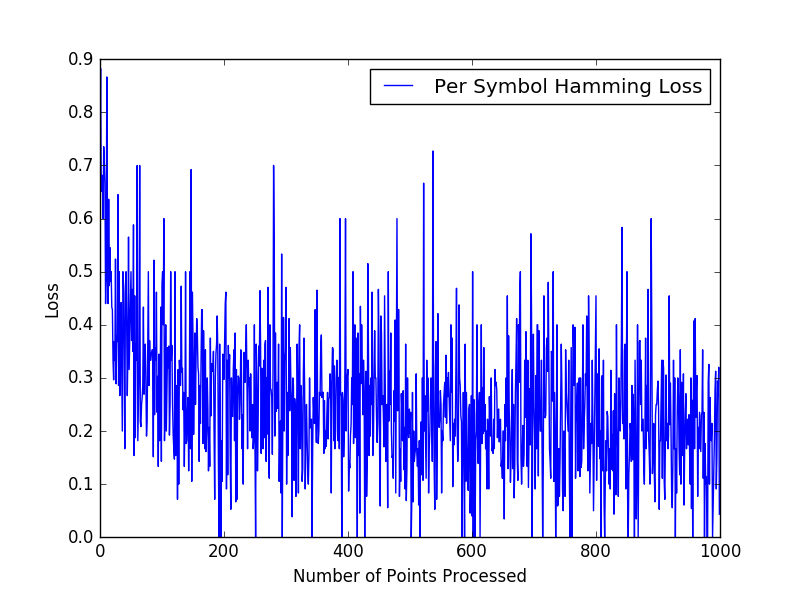
\includegraphics[width=5in]{hammingLoss1.png}
\caption{Hamming Loss for 10 passes with 100 points each pass}
\end{figure}

\begin{figure}[h]
\centering
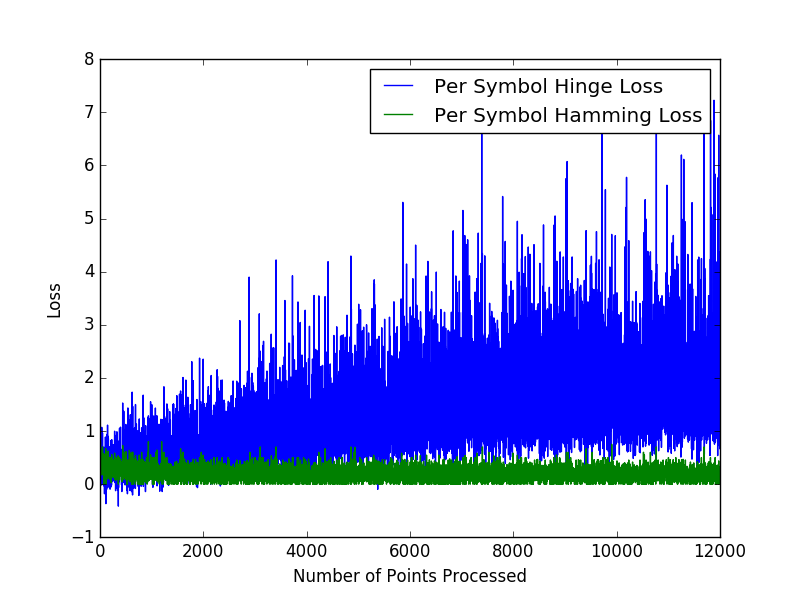
\includegraphics[width=5in]{hingeHammingLoss2.png}
\caption{Hinge and Hamming Loss for 2 passes with all points each pass}
\end{figure}

\begin{figure}[h]
\centering
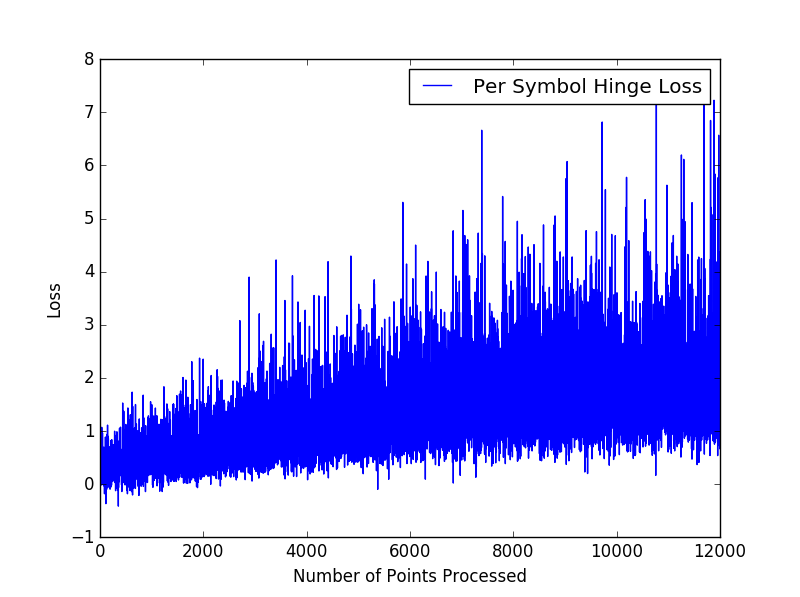
\includegraphics[width=5in]{hingeLoss2.png}
\caption{Hinge Loss for 2 passes with all points each pass}
\end{figure}

\begin{figure}[h]
\centering
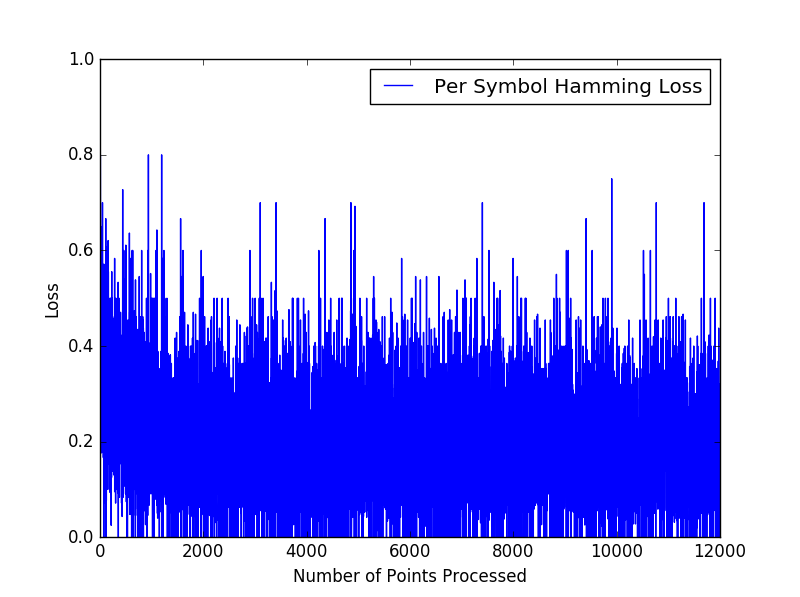
\includegraphics[width=5in]{hammingLoss2.png}
\caption{Hamming Loss for 2 passes with all points each pass}
\end{figure}



\end{document}
